\chapter{Implementacija i korisničko sučelje}
		
		
		\section{Korištene tehnologije i alati}
		
			Frontend aplikacije realiziran je pomoću \href{https://reactjs.org}{Reacta} korištenjem programskog jezika \href{https://www.javascript.com/}{Javascript}.  React je Javascript biblioteka otvorenog koda za izgradnju korisničkih sučelja temeljenih na komponentama korisničkog sučelja. Backend aplikacije ostvaren je pomoću \href{https://spring.io/projects/spring-boot/}{Spring Boota} zasnovanog na razvojnom okviru \href{https://spring.io}{Spring}, pisanog u programskom jeziku \href{https://www.java.com/en/}{Java}. Od razvojnih okolina korišteni su \href{https://code.visualstudio.com/}{Visual Studio Code} i \href{https://www.jetbrains.com/idea/}{IntelliJ IDEA}. Pri uspostavi arhitekture su također korišteni \href{https://render.com/}{Render}, \href{https://www.netlify.com/}{Netlify}, \href{https://tailwindcss.com/}{Tailwind CSS}, \href{https://docs.docker.com}{Docker Docs}, \href{https://axios-http.com/}{Axios}, \href{https://reactrouter.com/en/main}{React-Router-Dom} i \href{https://www.google.com/recaptcha/}{reCAPTCHA}. Baza podataka pisana je u \href{https://www.postgresql.org/}{PostgreSQL}. Za komunikaciju, dogovore i sastanke korišteni su \href{https://web.whatsapp.com/}{WhatsApp}, \href{https://www.microsoft.com/en-us/microsoft-teams/log-in}{Microsoft Teams} te \href{https://start.atlassian.com/}{Atlassian}. \href{https://www.lucidchart.com/pages/}{Lucidchart} je alat korišten za kreiranje dijagrama, a sama dokumentacija je pisana u markup jeziku \href{https://www.latex-project.org}{LaTeX} te uz pomoć alata \href{https://www.overleaf.com/}{Overleaf}. Udaljeni repozitorij projekta smješten je na web platformi \href{https://github.com/}{GitHub}.
			
			
			\eject 
		
	
		\section{Ispitivanje programskog rješenja}
			
			\textbf{\textit{dio 2. revizije}}\\
			
			 \textit{U ovom poglavlju je potrebno opisati provedbu ispitivanja implementiranih funkcionalnosti na razini komponenti i na razini cijelog sustava s prikazom odabranih ispitnih slučajeva. Studenti trebaju ispitati temeljnu funkcionalnost i rubne uvjete.}
	
			
			\subsection{Ispitivanje komponenti}
			\textit{Potrebno je provesti ispitivanje jedinica (engl. unit testing) nad razredima koji implementiraju temeljne funkcionalnosti. Razraditi \textbf{minimalno 6 ispitnih slučajeva} u kojima će se ispitati redovni slučajevi, rubni uvjeti te izazivanje pogreške (engl. exception throwing). Poželjno je stvoriti i ispitni slučaj koji koristi funkcionalnosti koje nisu implementirane. Potrebno je priložiti izvorni kôd svih ispitnih slučajeva te prikaz rezultata izvođenja ispita u razvojnom okruženju (prolaz/pad ispita). }
			
			
			
			\subsection{Ispitivanje sustava}
			
			 \textit{Potrebno je provesti i opisati ispitivanje sustava koristeći radni okvir Selenium\footnote{\url{https://www.seleniumhq.org/}}. Razraditi \textbf{minimalno 4 ispitna slučaja} u kojima će se ispitati redovni slučajevi, rubni uvjeti te poziv funkcionalnosti koja nije implementirana/izaziva pogrešku kako bi se vidjelo na koji način sustav reagira kada nešto nije u potpunosti ostvareno. Ispitni slučaj se treba sastojati od ulaza (npr. korisničko ime i lozinka), očekivanog izlaza ili rezultata, koraka ispitivanja i dobivenog izlaza ili rezultata.\\ }
			 
			 \textit{Izradu ispitnih slučajeva pomoću radnog okvira Selenium moguće je provesti pomoću jednog od sljedeća dva alata:}
			 \begin{itemize}
			 	\item \textit{dodatak za preglednik \textbf{Selenium IDE} - snimanje korisnikovih akcija radi automatskog ponavljanja ispita	}
			 	\item \textit{\textbf{Selenium WebDriver} - podrška za pisanje ispita u jezicima Java, C\#, PHP koristeći posebno programsko sučelje.}
			 \end{itemize}
		 	\textit{Detalji o korištenju alata Selenium bit će prikazani na posebnom predavanju tijekom semestra.}
			
			\eject 
		
		
		\section{Dijagram razmještaja}
			
			Dijagram razmještaja opisuje strukturu sustava, tj. odnose između sklopovskih i programskih dijelova. Donja slika predstavlja specifikacijski dijagram razmještaja, pri čemu se na poslužiteljskom računalu nalaze web aplikacija i baza podataka. Pristup aplikaciji klijenti ostvaruju putem web preglednika. Funkcioniranje sustava temelji se na modelu "klijent - poslužitelj", gdje klijenti zahtijevaju usluge od poslužitelja putem HTTP zahtjeva te očekuju odgovor. Poslužitelj obrađuje zahtjeve i šalje odgovore klijentima, a istovremeno upravlja komunikacijom s bazom podataka.

            \begin{figure}[H]
			         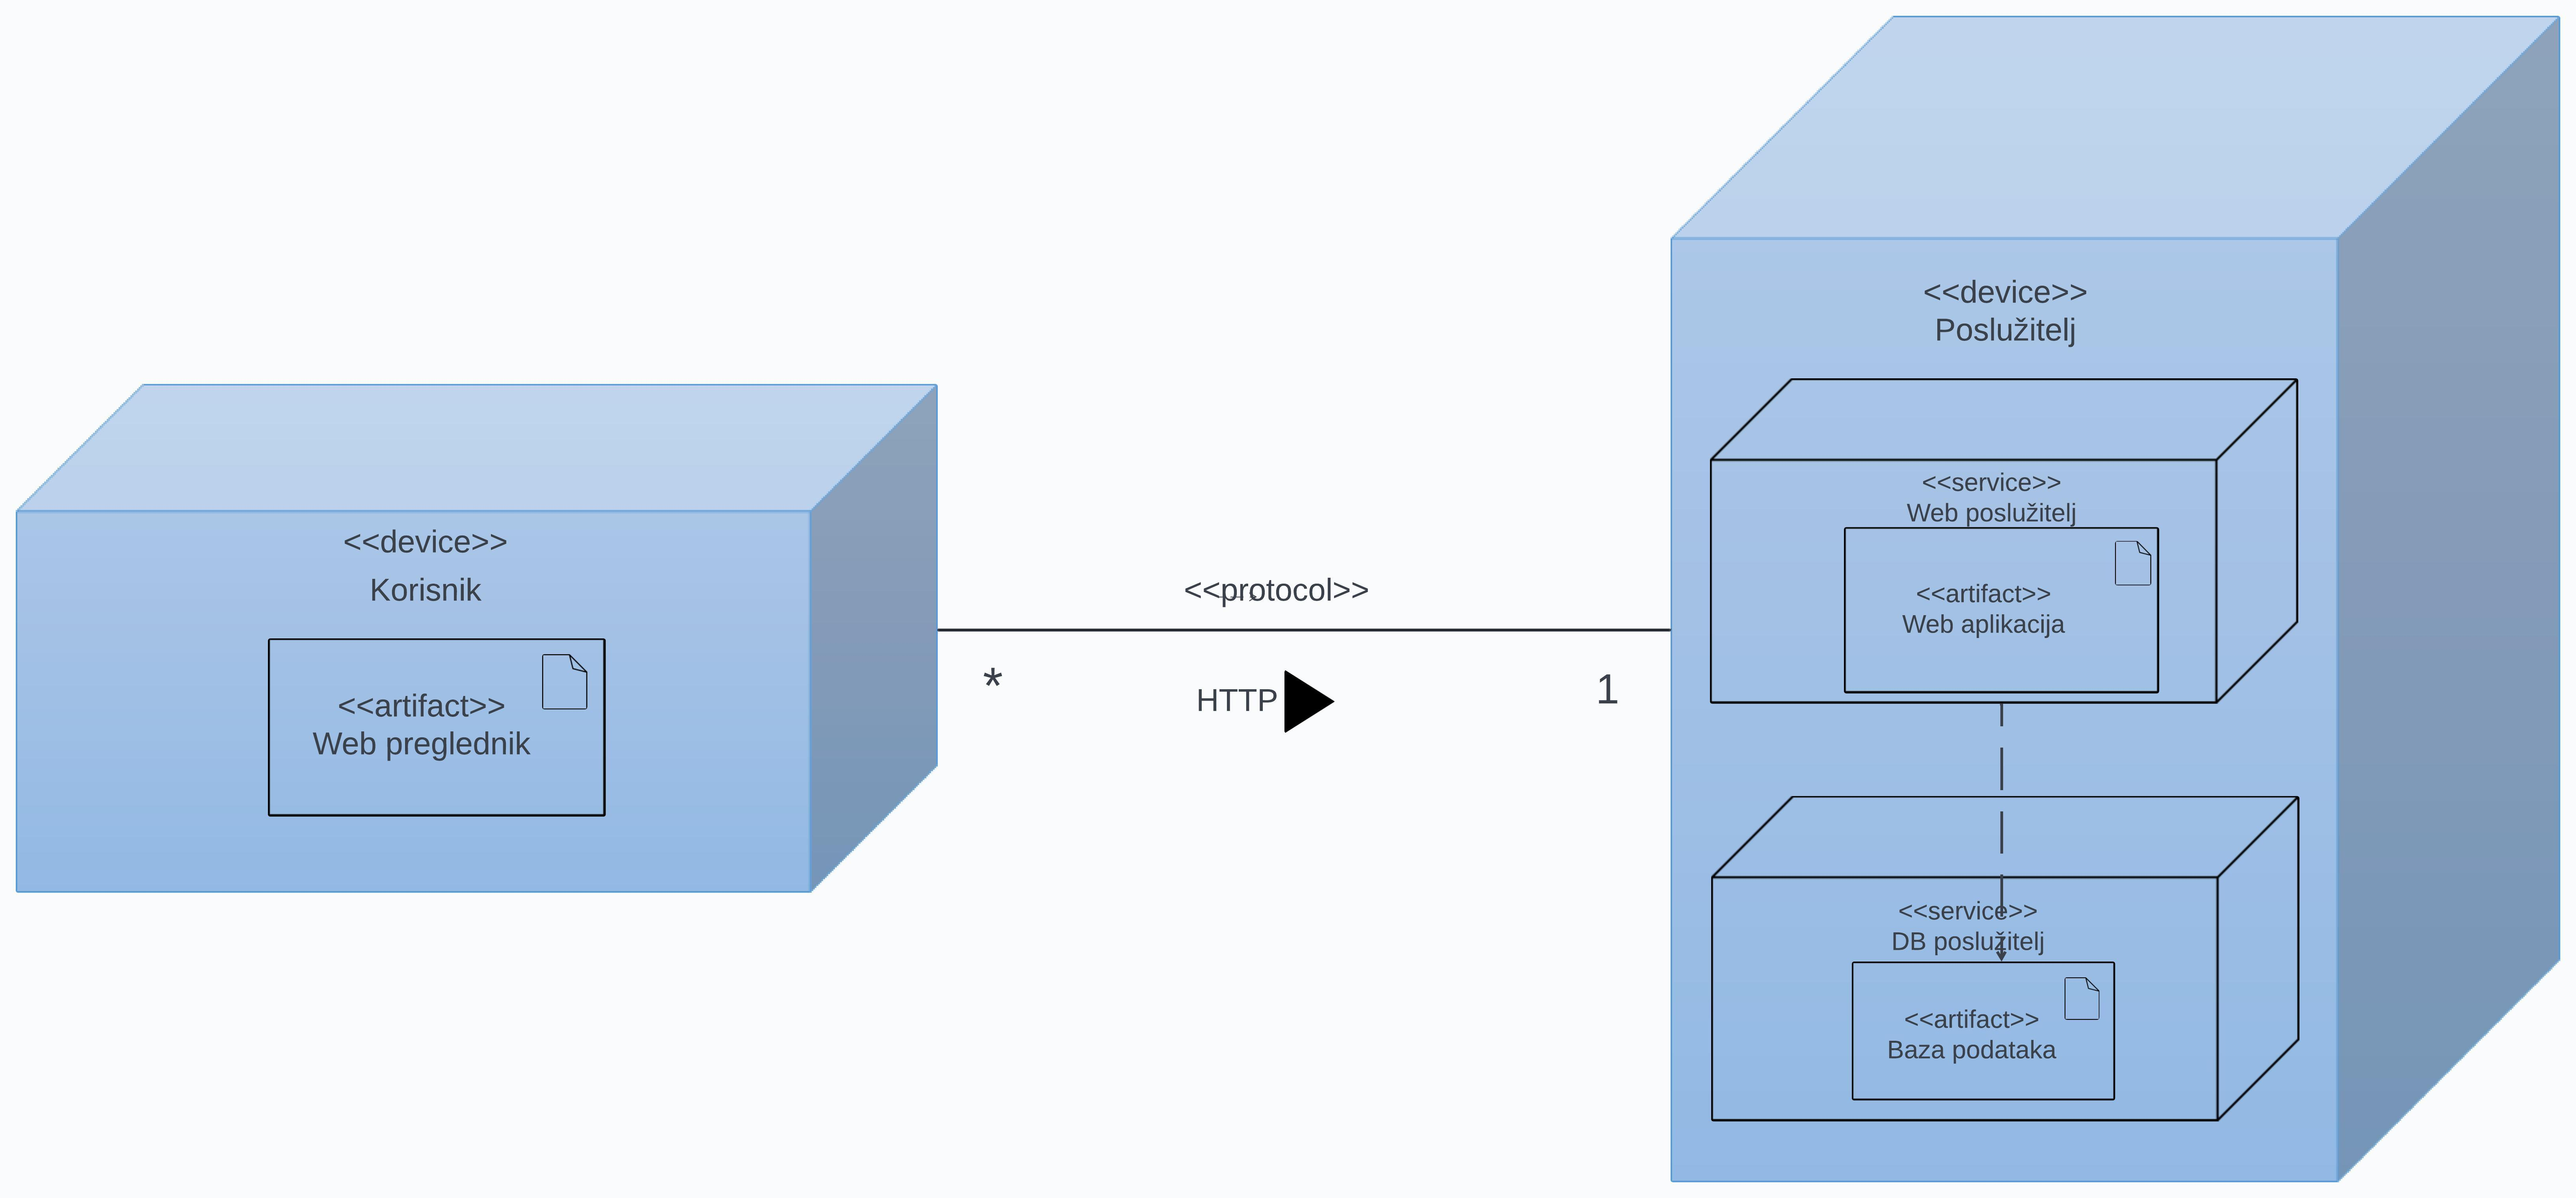
\includegraphics[scale=0.15]{dijagrami/Layout Diagram.jpeg}
			         \centering
			         \caption{Specifikacijski dijagram razmještaja}
			         \label{fig:LayoutDiagram}
		    \end{figure}
			
			\eject 
		
		\section{Upute za puštanje u pogon}
		
			\textbf{\textit{dio 2. revizije}}\\
		
			 \textit{U ovom poglavlju potrebno je dati upute za puštanje u pogon (engl. deployment) ostvarene aplikacije. Na primjer, za web aplikacije, opisati postupak kojim se od izvornog kôda dolazi do potpuno postavljene baze podataka i poslužitelja koji odgovara na upite korisnika. Za mobilnu aplikaciju, postupak kojim se aplikacija izgradi, te postavi na neku od trgovina. Za stolnu (engl. desktop) aplikaciju, postupak kojim se aplikacija instalira na računalo. Ukoliko mobilne i stolne aplikacije komuniciraju s poslužiteljem i/ili bazom podataka, opisati i postupak njihovog postavljanja. Pri izradi uputa preporučuje se \textbf{naglasiti korake instalacije uporabom natuknica} te koristiti što je više moguće \textbf{slike ekrana} (engl. screenshots) kako bi upute bile jasne i jednostavne za slijediti.}
			
			
			 \textit{Dovršenu aplikaciju potrebno je pokrenuti na javno dostupnom poslužitelju. Studentima se preporuča korištenje neke od sljedećih besplatnih usluga: \href{https://aws.amazon.com/}{Amazon AWS}, \href{https://azure.microsoft.com/en-us/}{Microsoft Azure} ili \href{https://www.heroku.com/}{Heroku}. Mobilne aplikacije trebaju biti objavljene na F-Droid, Google Play ili Amazon App trgovini.}
			
			
			\eject 